\documentclass{jsarticle}
\usepackage[dvipdfmx]{graphicx,color}
\begin{document}

\title{ALIS whitepaper}
\author{Masahiro Yasu and Sota Ishii and Takashi Mizusawa}
\maketitle

\section{目次}
\begin{itemize}
	\item ALISとは
	\item プラットフォームの紹介と特徴
	\item なぜ良質なコンテンツが集まるのか
	\item なぜ人々に価値を還元できるのか
	\item なぜALISは長期的な発展を続けることができるのか
	\item トークンはどのように作成・配布するのか
	\item 作成・配布のロジックはどのようなロジックなのか
	\item 不正はどうやって防ぐのか
	\item ALISの主要機能イメージ
	\item 技術的な優位性or技術面について * 入れるかどうか含めて検討
	\item どこにブロックチェーン技術を用いるのか
	\item チームのビジョン・ミッションおよびチームメンバーの詳細プロフィール
	\item プラットフォームのグロース戦略
	\item ファイナンシャル(ちょこっと戦略)
	\item お金の使い道
	\item 企業としての運営方針:透明化
	\item なぜ香港でICOを実施するのか
	\item 結論
\end{itemize}
\section{ALISとは}
ALISとは、日本初の分散型ソーシャルメディアプラットフォームである。従来のメディアと異なり、人々が認めるコンテンツを多くの個人が生み出す・発掘することを可能にする全く新しいソーシャルメディアである。正直に言うと、我々はSTEEM(https://steem.io)に大きな感銘を受けたところからこのプラットフォームの構想をスタートした。STEEMに関する情報に関しては、以下の記事が最もわかりやすいためぜひ参照してほしい。(https://xxx.xxx)具体的には我々のプロジェクトメンバーであるSota Ishiiが数枚の旅行の写真をSTEEMに掲載したことから始まる。なんとその記事はわずか一日で\$30近くの評価を得ることができ、我々は無事そのお金を使ってLPローンチ祝としてドミノの最高級ピザを購入することができた。我々は強烈な衝撃を受けるとともになぜこのような仕組みが実現出来ているのかを知りたくなり、徹底的にSTEEMを調べ上げた。そしてSTEEMを調べれば調べるほどその素晴らしさを知ることになった。STEEMはプラットフォーム自体が評価されることにより、STEEMのトークン自体の価値が向上しより高値でexchangeで取引されるようになる。その価値の上昇分がコンテンツのクリエイターおよび投票者に分配されることでこのような仕組みを実現していたのである。さらに、STEEMはトークンのみですでに\$3.78億(2017/7/9現在)の評価を得ている。新しいメディアの時代がやってきていることを身をもって体感した出来事であった。従来のメディアは収益源の多くを「広告」に頼っており(御存知の通り、googleもfacebookも収益の7割以上は広告収入である)、ユーザが記事やコンテンツを閲覧する際に広告を目にしたり、広告まがいの記事を目にすることはどうしても避けられない状態となっている。そのような状態に対して今まで広告業界においては様々な回避策が取られてきた。例えば積極的にユーザが広告を表示するとインセンティブを支払う仕組み、あるいは近年の機械学習によって本当にユーザが必要とする広告のみを配信する仕組み、など。今のところどれも成功しているようには見えず、相変わらずユーザは見たくない広告や、近年のコンテンツマーケティングの流行りを捉え違えた無意味なコンテンツ(広告に見えないから余計たちのわるい)を消費させられる立場にある。このような状況に対し、STEEMのスキームは先述の通りルールを根本から変えてしまうという力を持っている。しかしながらSTEEMには構造を革新できる素晴らしい面がある一方で、2つの大きな欠点があるように思えた(欠点があってもなおSTEEMは素晴らしいサービスであり、我々が大きなインスピレーションを彼らから得たことには変わりない)。一点目は、プラットフォームを支えるトークンの仕組みが複雑すぎてとても理解に時間がかかること。STEEMのみならず、STEEM SPやSTEEM Dollarsというトークンが存在し、入手のための方法も複雑であり、どのようなルールでプラットフォームが運営されているのかが初見のユーザには非常に理解が難しいものとなっている。これはリテラシーの低い新規ユーザを遠ざけるのに十分な理由になってしまい、メディアプラットフォームにおいて最も重要な要素の一つである新規ユーザ数と継続率に大きなマイナスを与えてしまう。二点目は、日本語対応がされていないこと。日本の経済力は世界第3位であり、未だに大きなマーケットであるといえる。一方で、常に「日本語」という言語の壁を抱えていることが原因で、グローバルプラットフォームから乗り遅れることが甚だしい(例えばWhatsApp, Tumblr, Pinterestなど、日本では存在すらほとんど知られていない)。しかしながら、だからこそ日本は狙うべきマーケットであると我々は捉えた。特にブロックチェーン技術に関しては欧米諸国が先陣を切っており、日本ではメインプレイヤーがほとんど存在しない。これは一度日本においてポジションを確立すれば、言語という壁が逆に強固なものになり独占的プレイヤーとしての立ち位置を確立することできる可能性を示唆している。また、言語の壁についてもMicrosoft社が同時通訳ツールをすでにリリースしているなど、あと5年もすればほとんど言語の壁を意識することがなくサービスを利用できる世界が来ると予想している。繰り返すことになるが、日本という世界的にみればニッチな世界で圧倒的なシェアを獲得し、言語の壁が崩れた際にグローバルマーケットに進出するという方法は合理的な競争戦略に則った方法であり、我々の成功確率を高めるものである。加えて、日本の国策として一億総活躍社会に基づいた働き方改革が推進されている(http://www.kantei.go.jp/jp/singi/hatarakikata/)。詳細は割愛するが、重要な施策の一つとして、人々の副業を推進するというものがある。なぜこの施策が重要視されるかを説明すると、日本という国家は世界で類を見ない高齢化社会になっており、圧倒的な労働人口不足にとらわれている。そのような中で、労働人口一人ひとりの生産性が最大化されているかというとそういうことはなく、もっと仕事を細切れにし企業の垣根を超えて個人が仕事をすることで生産性を向上させるという方法が模索されている。この推進を阻む大きな壁として「個人の信頼度がまったく可視化されていない」ということが挙げられる。ここに対して、最終的に我々はALISを通じて人の信頼を担保するというデータを与えることで、国策に紐付けた形でのエコシステムを完成させることを目論んでいる。以上に述べたように、我々は日本において、STEEMの良さを活かしつつ欠点も改良した新たなソーシャルメディアが成功し、最終的には人の信頼性を担保することができるプラットフォームへと進化することを確信し、このプロジェクトをスタートする決意を固めた。
★各ページに図を差し込みたい。LPのイラストと同じでも究極いい。
\section{プラットフォームの紹介と特徴}
ALISは、人々が良いと思うコンテンツを作成したクリエイターおよびそのようなコンテンツに投票をした人々に対して、より多くのALISトークンを配布するという報酬により信頼できるコンテンツ・人を発掘することができるソーシャルメディアプラットフォームである。そもそもこのようなメディア自体がかなり新しい概念のものになるため、STEEMと比較をした際の我々のプラットフォームの特徴を説明すると、1.我々のトークンは一つでシンプルであることにより、プラットフォーム発展のルールもシンプル化できること2.あえて仮想通貨の不安定性を許容し、インフレ率をSTEEMよりも抑えることで長期的なプラットフォーム維持を実現していること3.最終的なゴールを「人の信頼を可視化する」ことにおき、国策と紐付けて推進するというビジョンを持っている という3点である。それぞれの特徴については次章以降におって説明をしていく。
★3つのポイントを図で表現
\section{なぜ良質なコンテンツが集まるのか}
人々が良いと思うコンテンツを作り出す、もしくは投票するために必要なことは何であろうか。それは、より多くの人が認めるコンテンツを作り出すあるいは発掘した人に多くの報酬を支払うことである。コンテンツ作成者については、自分が作成したコンテンツがより多くの人に、かつよりALISトークンを多く持つ人に投票されることでより多くの報酬を得ることが可能になる。また、良質なコンテンツの発掘者に対しても、誰よりも早くかつ多くの人が良いと認めるコンテンツに投票することでより多くの報酬を得ることができる。これらに加えて、ALISトークンを多く持っている人であるほど報酬の量は線形で増えていく。つまり、よりALISトークンの報酬を得れば得るほど良質なコンテンツを生み出す or コンテンツを発掘するインセンティブが働き、更に良質なコンテンツが集まるというグッドスパイラルを形成することができる。これが良質なコンテンツが集まる理由である。このモデルをAARRRを元にしたシステム図に置き換えて説明しても同じことが言えることから、やはり報酬がプラットフォームの成長を加速させるキードライバーであることがわかる。★システム図の貼り付け
\section{なぜ人々に価値を還元できるのか}
我々のトークンはなんでもないただの電子データであり、それ単体では価値を持ち得ない。しかしながら、ALISのプラットフォームの価値があると認められれば認められるほどALISトークンが価値を持ち、取引所で高値で取引されるようになる。一見懐疑的に思われるかもしれないが、STEEMは同スキームですでに\$3.78億の評価を得ていることからこのスキームは実現可能であることが証明されている。また我々は基盤技術にブロックチェーンを利用しており、安価に高信頼のメディアを開発することができる。運営にコストがかからない分、より多くの価値をALISに貢献したメンバーに返すことができるということである。こちらも先述のAARRRをベースにしたシステム図から説明することができる。★システム図の貼り付け
\section{なぜALISは長期的な発展を続けることができるのか}
ALISが真に価値のあるプラットフォームとして認められるために最も重要なファクターがある。それは、ユーザーが粘着性を持ってずっと使い続けたいと思うプラットフォームを提供することである。そのための方法はいくつかあるが、一つのこだわりとしてトークンの性質を取り上げたい。我々のトークンは、ALISのプラットフォーム上で活用されている場合のインフレ率が50\%と高い。これは、昨今の仮想通貨が取引目的ばかりにexchangeで扱われていることに関する危機感から設定された数字である。ALISトークンを所有し、プラットフォームを発展させようと努力する人であればあるほどより多くのトークンを得ることができる仕組みづくりが重要である。しかしながら、この条件だけであればトークンをALISに預けたあと、増え次第すぐに引き出してexchangeで売るというインセンティブを防ぎ得ない。そこで我々ははXEMのPoIから着想し、トークンを移してから実効性をもつまでに時間が必要であるというロジックを導入する。具体的な式は以下である。
\begin{equation}
y = log_e(t-1) , t > 0
\end{equation}
ここでtはトークンをALIS上のwalletにうつしてから経過した時間である。上記数式を採用した理由は3点ある。1点目は、新規ユーザが早くALISの魅力に気づくことができるよう、tが小さいときには上昇幅が大きいということ。2点目は、長くユーザが使うことで100\%ALISのトークンの影響を受けることができるということ。3点目は、一度引き出してしまうとまたゼロから時間を経過させる必要があるため、簡単に引き出したくならないインセンティブをユーザに与えていることである。真にALISに貢献したいと思うユーザであればあるほどこの数式が合理性を持ち、長期的なプラットフォームの発展に貢献することができる。
\section{トークンはどのように作成・配布するのか}
ALISはICOによって資金を調達する予定であるが、preminedされた通貨になる。初期に500億枚を発行し、BticoinおよびEthereumとの交換を実施する。配布分の上限は250億枚であり、残りの250億枚については我々や我々のステークホルダーが所有することになる。我々が250億枚と全体の50\%を保有することには理由がある。一点目は我々が保有することで、我々自身がプラットフォームを発展させるという健全なインセンティブを持つということ。二点目は、状況に応じて我々が供給量をコントロールすることにより安定な価格を維持するということ。しかしながら、トークンの保有量を我々が最も抱えているからと言って、プラットフォームの価値を創造する決定権を我々が持っているということではないことにご留意いただきたい。加えて我々はこの所有トークンを無闇矢鱈に売ることはない(なぜなら配布量を増やすとトークンの価値が下がり、結果として我々はダメージを受けることになるからである。長期的な発展を見据えている我々がそのような行動をとる経済的合理性はどこにも存在しない)また、あくまでも良いコンテンツを作り出し、それを発掘するのはユーザである。そのようなユーザを集めるための戦略については別の章で後述する。ALISトークンはインフレ率が50\%のトークンであるとお伝えしたが、そのインフレ分がどのように配布されるかを説明する。基本的な思想は先述のとおり2点であり、1.素晴らしいコンテンツを作ったと認められた人に配布される 2.素晴らしいと人々が認めるコンテンツにいち早く投票した人に配布されるということである。この配布量について、ALISトークンの所有量が多ければ多いほど配布量を多く受け取れるというロジックを構築する。つまり、長くALISのプラットフォームに貢献をし、トークンを多く保有する人たちを最も重要なステークホルダーと捉え、彼らが力を持つことをルールとして設定する。これはPoIの仕組みに近しいものであり、プラットフォームが壊れてしまうと困る重要度の高いユーザであれば、健全なプラットフォーム運営を心がけるはずであるという前提に則っている。また、そうなると大量のALISトークンを買い占めたものが突然プラットフォームに参入し、プラットフォームの価値を自分の都合の良いものに変えてしまうのではないかという懸念が生まれるかと思う。この懸念に対しては、先述のPoIに着目した方法として、ALISトークンがプラットフォーム上で実際に有効になるまでには時間を要するという対応策を講じている。これがために大量のトークン所有のユーザがすぐに不正を働くことを防止しつつも、トークンをプラットフォーム上で保持し続けるというインセンティブも生むことができ一石二鳥の手法であるといえる。★図で誰にどれ位トークンが配布されるかを作りたい
\section{詳細の配布ロジックとパラメータの調整について}
まずALISの全体の発行量について言及しておこう。ALISは初期発行枚数としてX枚を予定しており、そのうちの最大X/2枚をcrowdsaleで販売する。1Ethereumあたり◯トークンのALISと交換予定なので、1トークンあたりの価格はYsatoshiである。さらに発行した分のうち、exchangeのwalletに入っている割合をx1,ALISwalletに入っている割合をx2とすると、x2に対して50\%のインフレ率が適用される。このインフレ率分のトークンが、コンテンツを投稿する人とコンテンツを評価する人に配布されることになる。この配布の詳細ロジックを述べるわけだが、まずは我々の原則の考え方を共有しておきたい。1. コンテンツ投稿者と投票者はどちらも尊重されるべきだが、コンテンツを製作するほうが労力がかかるためコンテンツ投稿者の割合を重くするべきである 2. コンテンツ投稿者は自分が投稿した記事がいいねを集めれば集めるほどコインを配布される。同様に、コンテンツ投票者は多くの人が良いねと予想する記事に投票するほどコインを配布される。 3. コインの配布量やロジックは、プラットフォームの発展に伴い変更すべきである 以上により、我々はインフレ分のALISトークンのうち、90\%をコンテンツ投稿者、10\%をコンテンツ投票者に配布するロジックを設定する(もし我々がICOの最低調達額3.5億円を達成した場合、1年目については投票者には6700万、投票者には750万円が全体で配布されることになる *ALISの価値が全く変動しないと仮定した場合。実際は価値が向上すると想定しているので配布量はもっと多くなると想定している)。これは、初期においては最も重要なことがコンテンツの量であると考えているからである。しかしながら、コンテンツの量が集まった次に重要な指標はコンテンツへの投票数に徐々に変わっていくだろう。その場合にはコンテンツ投票者への配布量を増やすべきであると考える。これらのパラメータについてはプラットフォームの段階に応じて調整されるべき値であると考えているが、その調整を我々運営者が実施するのは非常に中央集権的になってしまう。そこで、我々はコミュニティよりこのパラメータの調整を要望された場合、ALISトークンの所有量に応じた投票を実施し、コミュニティの総意(51\%以上の同意)を持ってパラメータを変更する運営方法を取りたい。
次に、投稿者・投票者一人ひとりに具体的にどのようにトークンが配布されるかを述べる。
まずベースとなるのはコンテンツに配布されるベースポイントAである。このベースポイントは投稿者・投票者それぞれの行動によって算出される。ALISトークンを多く保有している投稿者が投稿したコンテンツにはより多くのベースポイントが設定される。具体的には、 その人がもつ有効化されたALIS/ALIS上の総トークン数(if it is < 0.01, then set 0.01)が設定されることになる(イメージできない方もご安心いただきたい。後ほど簡単な図を使って説明を行う)。ここに、前回投稿時からの経過時間を加味した パラメータ 時間減衰(10分間はポイント0、その後時間が経つに連れて徐々に回復する)をかけた a1が投稿者ベースポイントとして設定される。 ALISを多く保有している人ほどプラットフォームを健全に保つインセンティブが働くことと、連続投稿したコンテンツに関しては不正の可能性が高いということを鑑みてこのような設定になっている。投稿者についても同様に、その人がもつ有効化されたALIS/ALIS上の総トークン数(if it is < 0.01, then set 0.01) * 時間減衰(5分間はポイント0、その後時間が経つに連れて徐々に回復する)= a2 をパラメータとして持っている。これらのユーザがいいね(α)もしくは低評価(β)をすることになるが、
α = Σai2 * ai3(a3 = 0 if 総投票数 < 10, else a3 = 1) * ai4( if user vote on his article) 
β = Σai2 * ai3(a3 = 0 if 総投票数 < 10, else a3 = 1) * ai4( if user vote on his article) 
* i = ブロック生成時間の間にその記事に対して投票を行った全ユーザ
として計算される。最後に、ベースポイントを計算する式は以下となる
An = a1 + (α - β)(if An < 0 then An = 0,  and α < β, An=0)
* n = 当該時間内に投稿されたある記事
αに関してはα*( An / An + β )が自分のその記事に対するいいねポイントになり、ベータに関してはβ*2が自分の評価ポイントになる。
★懸念はこうすると低評価のほうがポイントを貰えるので増えてしまうかもということ。要検討。雑な低評価をした時のリスクが高くなるように設定するか、いいねと低評価の重み付けを同じにするか。後者のほうが筋が良さそう。
あとの計算は簡単である。投稿者は自分のコンテンツポイント/総コンテンツポイント * インフレ分ALIS * 0.9を受け取り、投票者は自分の投稿ポイント/総投稿ポイント * インフレ分ALIS * 0.1を受け取ることになる。説明が数式ばかりで難解だと思われる方のために、単純化したシチュエーションで図を用いて説明する。
★トークン配布の図を準備する
\section{不正はどうやって防ぐのか}
上述の配布ロジックに従うと、トークン取得に関して次のような不正をユーザに許し、大多数のユーザが不利益を被ってしまう可能性がある。1.ユーザが複数のダミーアカウントを作成し、自身が作成したコンテンツに積極的に投票を行うことによるALISトークンの取得 2.特定のユーザが結託をし、指定したコンテンツに対して積極的に投資をしトークンを取得する 我々はこれらの不正を防ぐための策をすでに用意してある。まず1.に関しては容易にダミーアカウントを作成出来ないような対策を行う。具体的にはSMSによる本人確認認証もしくは、facebookアカウント連携による登録導線のいずれかにて対応を行う。また、2点目に関しては、1. 特定ユーザがあるコンテンツに投稿し、時間をあけずに別のコンテンツに投稿した場合はそのコンテンツの投票に対する評価は無効とする(なぜなら、そんなに短期間でいくつものコンテンツを読みうるユーザのほうが統計学的には少ないはずだからである)、Bad評価をされたコンテンツのBa評価の割合を見て、不正を働いていると思しきユーザへの配布量を抑える、などの対応により不正に対処していく。これはSTEEMがすでに採用している不正防止ロジックから着想を得たものであり、STEEM自体がうまく動いていることから我々のプラットフォームでもうまく動作することが期待される。
\section{ALISの主要機能イメージ}
本章ではALISの持つ機能概要についてお伝えする。機能の細かい説明については各章にて述べているため、本章で説明するのはあくまでも重要な機能に絞って、イメージをお伝えすることとしたい。1.コンテンツ一覧のWF 2.ユーザが投稿できる内容の2つについて絞ってお伝えすることとする。基本的にはsteem( https://steemit.com )と似た画面イメージになると考えてもらって良い。★ALISのWFのイメージを作りたい。最大のPRポイントは「信頼度の高い人のポスト」と人経由でも記事をたどることができること。
\section{技術的な優位性or技術面について * 入れるかどうか含めて検討}
coming soon
\section{どこにブロックチェーン技術を用いるのか}
我々はブロックチェーン技術を次の用途に用いる。ユーザが投稿したコンテンツの内容および、そのコンテンツに対するユーザの評価データの保存。具体的にはALISコインを入れharvestedされたwalletを持つユーザは、それだけでPoSに参加することができる。このPosが行っている作業の中身は、先述のトークン配布のためのポイントを計算し、各ユーザに適切に配布することである。我々はコンテンツの削除や修正を容易には許さない仕組みにするためにこの方法を取る。なぜなら、削除や改竄を許してしまうと、信頼性の高いコンテンツを書くというモチベーションに多少なりとも悪影響を及ぼすことになるからである。もちろん、こうすることによるデメリットとしてユーザが気軽に投稿できなくなるという点も存在する。その点については、削除や修正はできないが、追記は可能という形で回避する予定である。また、ブロックチェーン技術を用いることで従来のSNSにおいては大量に必要であった運用コストが、同等の信頼度を実現する場合に信じがたいほどの低コストで運用することができるようになる。我々は現在、EthereumやMicrosoft Azure(我々は現在Azure BizSparkパートナーとしてMS社から認定されており、BizSpark+としての審査も受けることになっている。)などの技術のうち、どの技術が最も高信頼・低コストを実現できるかを検討中である。本章についてはまだ技術的な検討が完了していないため、追加の情報が出次第追記していくことを約束する。
\section{チームのビジョン・ミッションおよびチームメンバーの詳細プロフィール}
我々ALISのチームのビジョン・ミッションは明確である。ビジョンは、世の中の有益な情報と人を可視化することにより、CtoCでの経済圏の成長スピードを加速させることである。日本という国家においては、人口減少が国家問題として重くのしかかっている。この重しを取っ払うためには国民一人ひとりの生産性を向上させることが必須であり、国としても一億総活躍社会というビジョンを掲げ、働き方改革というミッションを遂行している段階にある。国民一人ひとりの生産性を向上させるには様々な方法があるが、もっとも重要なことの一つは「一人の人間が関わる仕事の幅を増やすこと」である。いわゆる副業と呼ばれるこの方法は現在日本において積極的に推進しようという動きが加速しているが大きな問題がある。それは、一個人が仕事をすることになる以上、一個人の信頼性を担保しないことには結局は絵に書いた餅で終わってしまうことである。我々はこの問題に対して、信頼できるコンテンツと人との出会いというネットワーキングを通じ、解決するような方法がないかを考えていた。その折にSTEEMに出会い、このようなソーシャルメディアを構築することが本当に一個人が信頼性を持つための近道ではないかと思いこのプロジェクトをスタートした。つまり我々のミッションは、1.報酬によって有益な情報・人と無益な情報・人とを区別することができる2.どんなに信用がない個人でも、有益なコンテンツを創造あるいは発掘した個人に信用を付与すること3.それを人々が自律的な経済圏で営めるプラットフォームを容易することである。ビジョンに対して真っ直ぐな思いをもった我々であるからこそ成し遂げられると自負しているし、我々がやるべきだという使命感を抱いている。
★チームメンバーについても紹介をしたい。メンバーのプロフィール+ストレングスファインダーあたりを乗せる。プロフィールはLPとは違う感じで、もっと人となりが伝わるような形で。
\section{プラットフォームのグロース戦略}
私Masahiro Yasuはかつて日本におけるビジネスSNS(Linkedinと似た立ち位置のもの)を開発していた経験がある。その経験から考える、プラットフォームをグロースさせるのに最も大事な要素の一つは「ユーザからのフィードバック」である。この重要性はFacebookやInstagramなどのSNSを使っているユーザであればわかると思うが、いかに自分の友人・知人に関する情報や自分が投稿したものに対して通知を通じてフィードバック数を増やすということを彼らが行っているかという事実からもわかると思う。結局は自分が投稿したコンテンツに対して、いかに人々が反応してくれるかがプラットフォーム継続のために最も重要なファクターなのである。幸運なことに、この課題はトークン配布ロジックを実現することで解決することができる。つまり、人々は「まだ誰も評価してないが、将来評価しうるコンテンツを真っ先に見つけ出し、自分がいちばん最初にいいねをすること」という行動原理にのっとって動くと想定されるからである。これは報酬が伴うALISならではのユニークな解決方法であり、経済ルールにすでに埋め込まれているという協力なものであることに留意いただきたい。また、グロースのための要因として見過ごされがちであるが、現在大きくグロースしているfacebookやかつて日本で大盛況をしたmixiに共通な条件として、「いかに内輪から始めるか」ということがある。これがグロースのために重要だと我々が考える2点目の要素だ。facebookはハーバード大学のコミュニティーツールとして、mixiは日本の大学のツールとしてどれも「内輪感」からスタートしているということが重要である。実は多くのSNSがこのような内輪感からスタートしているかが少し調査するだけでおわかりいただけるかと思う。我々はこの重要性を担保するために、まずは「仮想通貨・トークンに興味がある人々」をターゲットとしてコンテンツを増やしていくという戦略を取りたい。理由は明快である。1.仮想通貨に関する情報はどれも信頼性の低いものが溢れており、人々は信頼のおける情報ソースを求めている2.仮想通貨に関する情報はどれもクオリティの低い情報ばかりであり、役に立たない(ご都合主義のテクニカル分析を見せつけられ、○○は上がるぞ!!というtwitterを見て涙したユーザは何人いるだろうか。安心してほしい、私もその一員である)3.誰もが仮想通貨の投資でマイナスを蒙りたくないと考えている4.何より我々が仮想通貨・トークンが大好きであり、最も情熱を持って打ち込めるコンテンツであるからである。上述を踏まえたグロース戦略の大観をお伝えすると以下2点になる。1.ニッチな領域×高信頼度を必要とするユーザが多い分野(初期は仮想通貨を想定)において、ユーザ集客を効率的に実施する 2.そのようなユーザが参加後から多くのフィードバックを受けることができる仕組みを準備する(タグ指定による新規コンテンツの通知アラート、自分の投稿に対するコメントの通知アラート、など)初期はあくまでもコンテンツ量が重要なため、良質なコンテンツの投稿者に多くのトークンが配布されるロジックを組み込む。しかしながらプラットフォームがグロースするに連れてこの割合は変更されるべきものであると我々は感じている。時々のグロースタイミングに適切なキードライバーが最大となるように報酬の割合に関するパラメータ調整を実施したいが、それを我々が行ってしまうと中央集権的になってしまう。よって、先述の通りALISトークンを保有するユーザによる投票でどのようにパラメータを調整するかを決定したいと考えている。★システム図を添付する
\section{ファイナンシャル}
トークンが将来どれぐらいの価値になるのかを楽観・中庸・悲観の3パターンで記載する。算出にあたってSTEEMの現在の評価価値を大いに参考にさせていただいた。基本的なロジックとしては、STEEMにおける1ユーザの価値を参考に、我々のユーザ数の伸びにその価値をかけるという方法で算出した。ここで暗黙の前提としておいている以下の点にご注意いただきたい。1.1ユーザが平均2投稿をする(STEEMのユーザ平均値)2.ユーザ数以外のあらゆる部分(運営メンバー、アプリケーションの素晴らしさ、利用ユーザの国など)はSTEEMと同等 ここで算出した3年後の価値を、3年後に発行されているALISトークンの総量で割ったものが1ALISトークンあたりの価値になる。算出のために用いた数字はすべて下記に掲載したのでご参考いただきたい。
	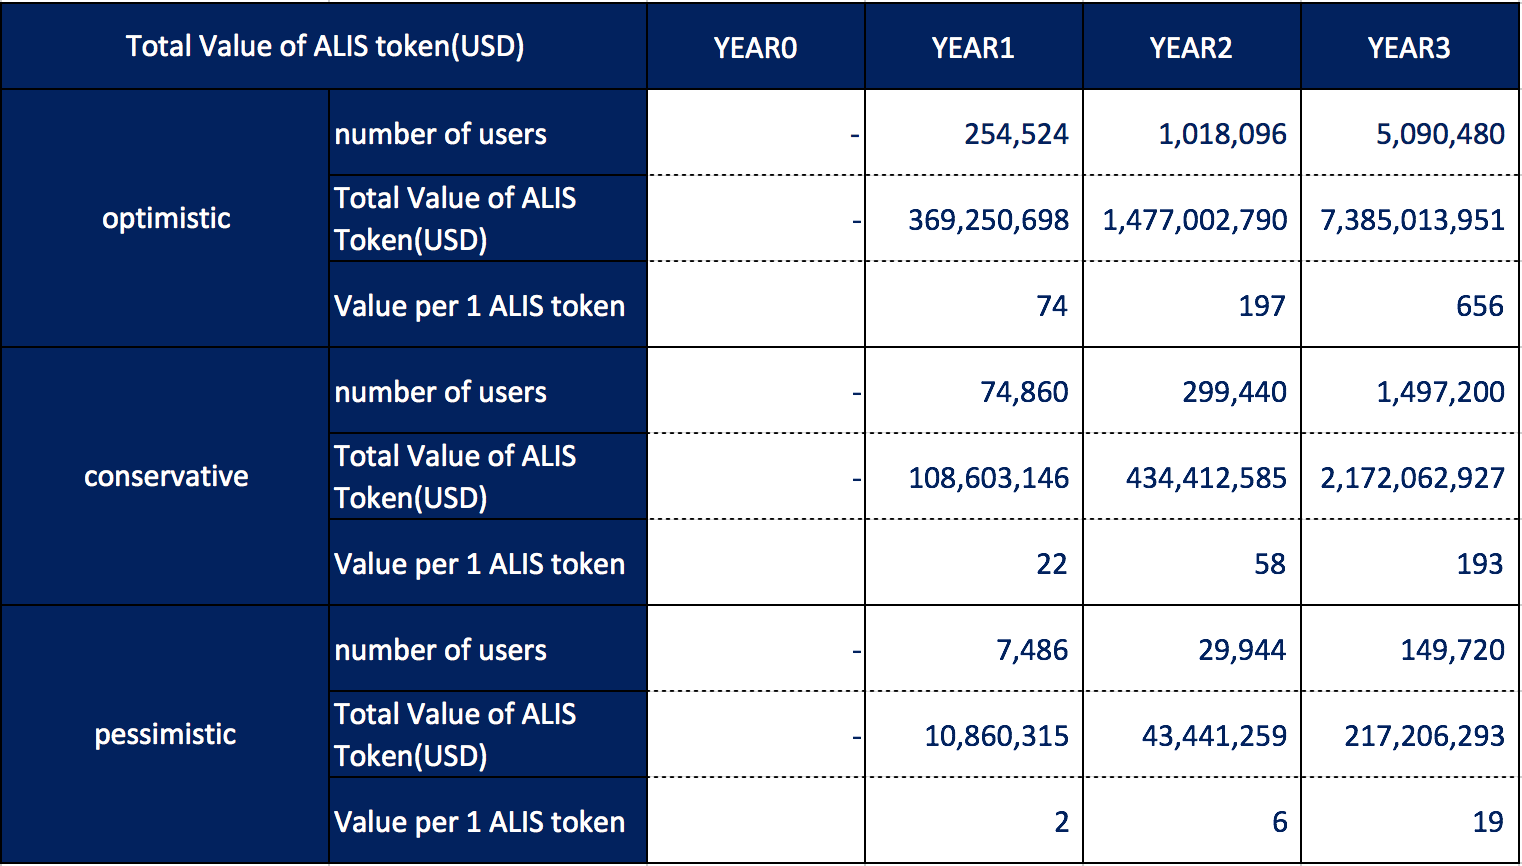
\includegraphics[scale=0.6]{img/financialtable.png}
\section{お金の使い道}
我々はクラウドセールの最低目標額3.5億を集めた場合、トークンを以下のような用途・割合で使う想定でいる。1. 25\%:優秀な開発メンバーのアサイン(特に優秀なUI/UXデザイナー1名、WEBデザイナー1名、フルスタックエンジニア4名。)2. 25\%: ユーザ集客のためのマーケティング費用 3. 25\%: 国内事業者として認可されるための申請費用 4.25\%:初期に協力してくれたメンバーや今後協力してくれるパートナーに対する費用 3.5億円の調達をオーバーした分に関しては、基本的にはマーケティング費用にほとんどを投じるが以下のような用途にも使用する可能性がある。 ・より強いバックオフィス(経理・法務)の構築 ・固定のオフィスの準備(我々はなるべく固定費を持たないために、資金に余裕が出るまでは固定のオフィスはレンタルしない想定でいる。少しでもプロジェクトの成功確率を高めるためである)

	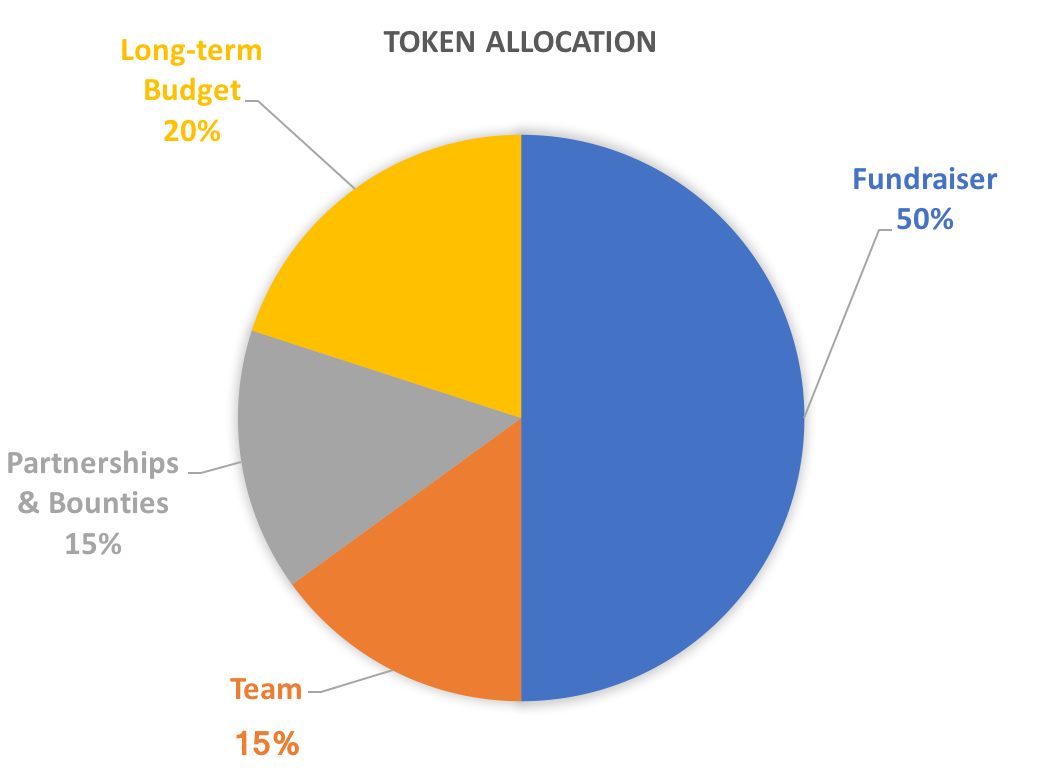
\includegraphics[scale=0.4]{img/tokenallocation.png}
	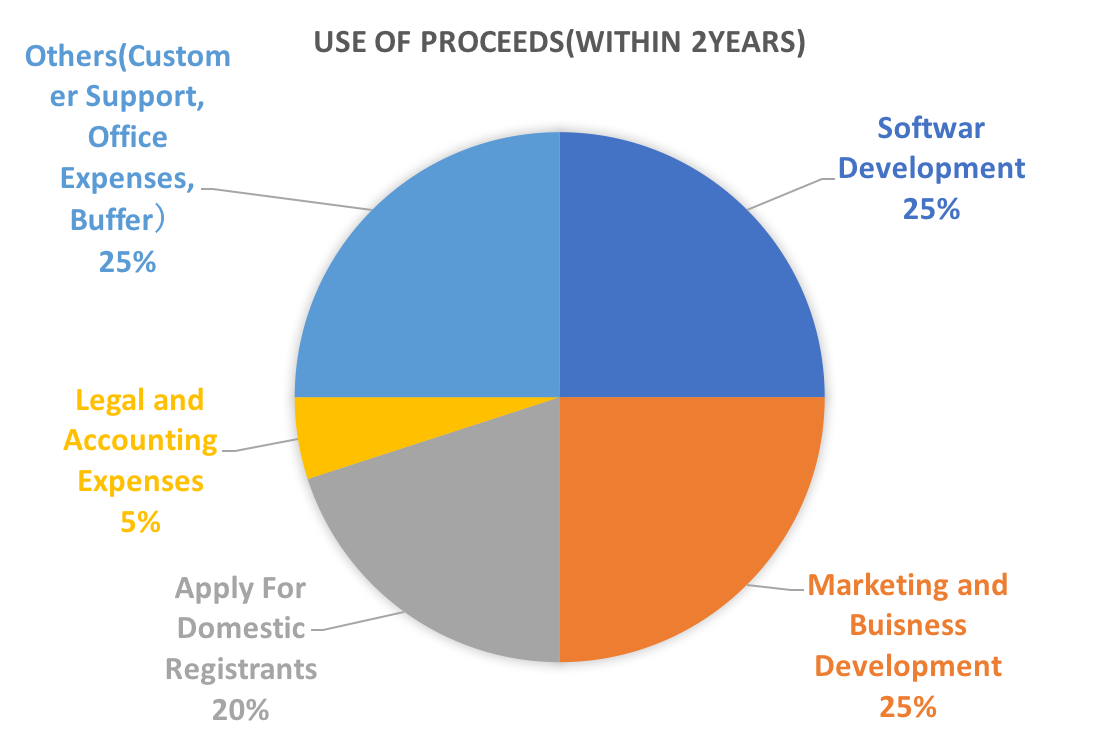
\includegraphics[scale=0.4]{img/useofproceeds.png}
\section{企業の運営方針}
我々は現在の株式会社はとても旧世代なものであると感じる。まずチグハグな点がすごく多い。会社は株主のものと言いながらも、株主が知ることができる情報は株主総会での着飾れた情報のみである。またその経営権を託されている役員人は、自分が絶対正解だという前提の元でしか決定をくたさず、現場社員にその決定を押し付けている。ゲイリー・ハメルが未来の経営でも書いているように、会社のシステムは数百年以上進化を止め化石化しており、我々はこの状況に1石を投じるべく以下のようなルールで経営をしていきたい。1.プロジェクトの状況はtrelloなどを用いてすべて透明化する2.メンバー間のコミュニケーションについてもできるだけ公開する3.開発コードはすべてオープンソースとしてgithubに公開する4.会社の方向性およびメディアのグランドルール変更については、トークンを所有する人の多数決にて承認とする5.働く従業員の給与は従業員間ですべて公開する。 どこまでこのルールを突き詰めて運用できるかは分からないが、なるべく次世代の経営に挑戦し、本当に会社を支えてくださる人々と一緒に運営できる組織づくりを目指したい。
	
\includegraphics[scale=0.4]{img/thefutureofmanagement.jpg}
\section{なぜ香港でICOを行うのか}
我々が日本でプラットフォームを開発するにもかかわらず、香港でICOを行うことに不安を覚える方が少なくないと察する。理由は明確で、日本においては2017年4月以降国内事業者のICOが「改正資金決済法」(https://xxx.xxx)の施行に伴い禁止されたからである。我々も当初は日本でのICOを想定していたが、最近の国会での討論(http://xxx.xxx)なども踏まえ日本におけるICOは違憲に当たる可能性が高いと判断し、海外でICOを実施することを決断した。その中でも香港を選んだ理由については、最もコストを安く会社を設立・維持できる国であり、なおかつ仮想通貨に関する規制がないことが大きな要因である。香港で調達したトークンを元に、日本国内における登録事業者申請を行うことで国内ユーザも海外ユーザもなんの柵もなくトークンが取引できる状態を目指す。また、国内事業者になることで日本国内の仮想通貨取引所に取り扱ってもらうことができるという大きなメリットが生まれる。我々は国内最大級の取引所とすでにコンタクトを取っており、将来の上場可能性と方法についても議論をしている。この事業者申請が完了するまでは、海外の取引所においてのみ取引可能なトークンとなることをご留意いただきたい。また、香港の法人については当面ICO目的のためのみに存在する法人として扱うが、日本の法律問題やその他の問題で日本法人での運営が難しい部分が出てきた際にバックアップする存在として長期的に維持していく想定でいる。
\section{結論}
長々と付き合ってくださったことに感謝をお伝えする。お読みいただいたとおり、我々は本気でこのプラットフォームの実現に燃えている。自分たちの理想的な世界を実現するまたとないチャンスであり、なおかつそれを経済的ルールに限りなく縛られずにやれるチャンスであると考えているからである。もしこの世界の実現に賛同してくださるのであれば、ぜひともICOにご参加いただきプラットフォームの発展に貢献いただきたい。我々は、皆様と新たなプラットフォームを構築できる日が来るのを楽しみに待つこととし、このホワイトペーパーを締めくくる。
\end{document}
